% =====================================================================
%  RetailForge — Devpost Hackathon Presentation
%  Macy's-inspired theme (red star, editorial serif, black/white)
%  Compile:  latexmk -pdf retailforge.tex     (or run pdflatex twice)
% =====================================================================
\documentclass[aspectratio=169,11pt]{beamer}

\usepackage[T1]{fontenc}
\usepackage[utf8]{inputenc}
\usepackage{charter}              % editorial serif (department-store feel)
\usepackage{microtype}
\usepackage{booktabs}
\usepackage{colortbl}
\usepackage{tikz}
\usetikzlibrary{shapes.geometric,arrows.meta,positioning,calc,backgrounds,fit}
\usepackage{graphicx}

\graphicspath{{../screenshots/}{../diagrams/}}

% ---------- Macy's palette --------------------------------------------
\definecolor{macyred}{HTML}{E11B30}
\definecolor{macydark}{HTML}{A00C1D}
\definecolor{macydeep}{HTML}{5F0911}
\definecolor{ink}{HTML}{0A0A0A}
\definecolor{ink70}{HTML}{2B2B2B}
\definecolor{surface}{HTML}{F6F6F6}
\definecolor{line}{HTML}{E5E5E5}
\definecolor{gold}{HTML}{F5A623}

% ---------- Beamer theming --------------------------------------------
\usetheme{default}
\usefonttheme{serif}
\setbeamertemplate{navigation symbols}{}
\setbeamercolor{normal text}{fg=ink}
\setbeamercolor{structure}{fg=macyred}
\setbeamercolor{frametitle}{fg=white,bg=macyred}
\setbeamercolor{itemize item}{fg=macyred}
\setbeamercolor{itemize subitem}{fg=macydark}
\setbeamercolor{block title}{fg=white,bg=macyred}
\setbeamercolor{block body}{fg=ink,bg=surface}
\setbeamerfont{frametitle}{series=\bfseries}
\setbeamerfont{title}{series=\bfseries}
\setbeamertemplate{itemize item}{\small\textbullet}

% Frame title as a slim red band with a star tick
\setbeamertemplate{frametitle}{%
  \nointerlineskip
  \begin{beamercolorbox}[wd=\paperwidth,ht=2.4ex,dp=1.1ex,leftskip=0.6cm,rightskip=0.6cm]{frametitle}%
    \raisebox{0.1ex}{\tikz{\node[star,star points=5,star point ratio=2.3,fill=white,
        inner sep=1.1pt]{};}}\hspace{4pt}%
    \strut\insertframetitle%
  \end{beamercolorbox}%
}

% Footer: page number + wordmark
\setbeamertemplate{footline}{%
  \hbox to\paperwidth{\hspace*{0.6cm}\color{ink70}\scriptsize
    \textcolor{macyred}{$\star$}\,\textbf{RetailForge}\hfill
    Multi-Agent Retail Intelligence\hfill
    \insertframenumber\hspace*{0.6cm}}%
  \vskip4pt
}

% ---------- Reusable star command -------------------------------------
\newcommand{\macystar}[2][macyred]{\tikz{\node[star,star points=5,
  star point ratio=2.3,fill=#1,draw=#1,inner sep=#2]{};}}

% ---------- Title-style full-bleed red frame --------------------------
\newcommand{\titlestar}{\tikz{\node[star,star points=5,star point ratio=2.3,
  fill=white,draw=white,inner sep=10pt]{};}}

\begin{document}

% ===================== 1. TITLE ======================================
{%
\setbeamertemplate{footline}{}
\begin{frame}[plain]

\begin{tikzpicture}[remember picture,overlay]
  \fill[macyred] (current page.south west) rectangle (current page.north east);
  \fill[macydeep,opacity=0.55] (current page.south west) rectangle
        ([yshift=2.4cm]current page.south east);
  \node[anchor=north west,white] at ([xshift=1.1cm,yshift=-1.0cm]current page.north west)
      {\titlestar};
  \node[anchor=west,white,font=\Huge\bfseries] at
      ([xshift=4.0cm,yshift=-1.7cm]current page.north west) {RetailForge};
  \node[anchor=west,white,font=\large] at
      ([xshift=4.02cm,yshift=-2.65cm]current page.north west)
      {Your AI Personal Shopper --- that actually shops.};
  \node[anchor=west,white,font=\normalsize] at
      ([xshift=1.15cm,yshift=0.3cm]current page.west)
      {\parbox{10.5cm}{\raggedright A production-grade \textbf{multi-agent retail
       intelligence} system: a department-store storefront with a concierge that
       searches, recommends, builds discounted kits, places orders and issues
       refunds --- with safe, gated access to live data.}};
  \node[anchor=west,white,font=\footnotesize] at
      ([xshift=1.15cm,yshift=-1.4cm]current page.west)
      {\parbox{11cm}{\raggedright \textbf{Live demo:}
       retailforge-frontend-awghszkm2a-uc.a.run.app}};
  \node[anchor=south west,white,font=\scriptsize] at
      ([xshift=1.15cm,yshift=1.25cm]current page.south west)
      {Google ADK \ $\cdot$\ Gemini 2.5 Flash \ $\cdot$\ MCP Toolbox \ $\cdot$\ MongoDB
       Atlas Vector Search \ $\cdot$\ Cloud Run};
  \node[anchor=south west,white,font=\scriptsize\itshape] at
      ([xshift=1.15cm,yshift=0.55cm]current page.south west) {Devpost Hackathon Submission};
\end{tikzpicture}
\end{frame}
}

% ===================== 2. PROBLEM ====================================
\begin{frame}{The problem}
\begin{columns}[T]
\begin{column}{0.5\textwidth}
  \textbf{\color{macyred}Retail chatbots answer. They don't act.}
  \begin{itemize}
    \item Shoppers get text replies, then still hunt, compare and check out alone.
    \item "Recommendations" rarely know real \textit{stock}, \textit{price} or \textit{promotions}.
    \item Bundling and discounts are manual work the shopper does in their head.
  \end{itemize}
\end{column}
\begin{column}{0.5\textwidth}
  \textbf{\color{macyred}Letting an LLM touch the database is risky.}
  \begin{itemize}
    \item Direct DB access = an agent one hallucination away from a destructive write.
    \item Hard to audit \emph{what} an agent actually did to your data.
    \item No clean contract between "the model" and "the system of record".
  \end{itemize}
\end{column}
\end{columns}
\vfill
\begin{block}{The gap}
We need a concierge that \textbf{takes real, correct actions} on live retail data ---
\emph{and} a safety boundary that makes those actions auditable and impossible to abuse.
\end{block}
\end{frame}

% ===================== 3. WHAT IT DOES ===============================
\begin{frame}{What RetailForge does}
A shopper chats with one \textbf{Personal Shopper}. Behind it, a team of specialist
agents do the work --- end to end.
\vspace{0.4em}
\begin{columns}[T]
\begin{column}{0.5\textwidth}
\begin{itemize}
  \item \textbf{Find} --- natural-language semantic search over the catalog (vector embeddings).
  \item \textbf{Recommend} --- "also bought", trending, and history-aware picks.
  \item \textbf{Support} --- order status, cancellations, refunds.
\end{itemize}
\end{column}
\begin{column}{0.5\textwidth}
\begin{itemize}
  \item \textbf{Build a kit} --- assemble a multi-category bundle for an activity\dots
  \item \textbf{\dots and discount it} --- auto-pick the best valid promotion.
  \item \textbf{Check out} --- place the order \& decrement inventory for real.
\end{itemize}
\end{column}
\end{columns}
\vfill
\begin{center}
\setlength{\fboxsep}{6pt}\setlength{\fboxrule}{0pt}%
\colorbox{surface}{\parbox{0.92\textwidth}{\centering
\textit{"Build me a weekend camping kit under \$300 with a discount"} $\Rightarrow$
the concierge routes to the Billing agent, searches across categories, checks stock,
applies a promo, and returns a ready-to-buy bundle.}}
\end{center}
\end{frame}

% ===================== 4. LIVE STOREFRONT ============================
\begin{frame}{The storefront --- live on Cloud Run}
\begin{columns}[c]
\begin{column}{0.62\textwidth}
  \begin{tikzpicture}
    \node[inner sep=0,draw=line,line width=0.6pt] {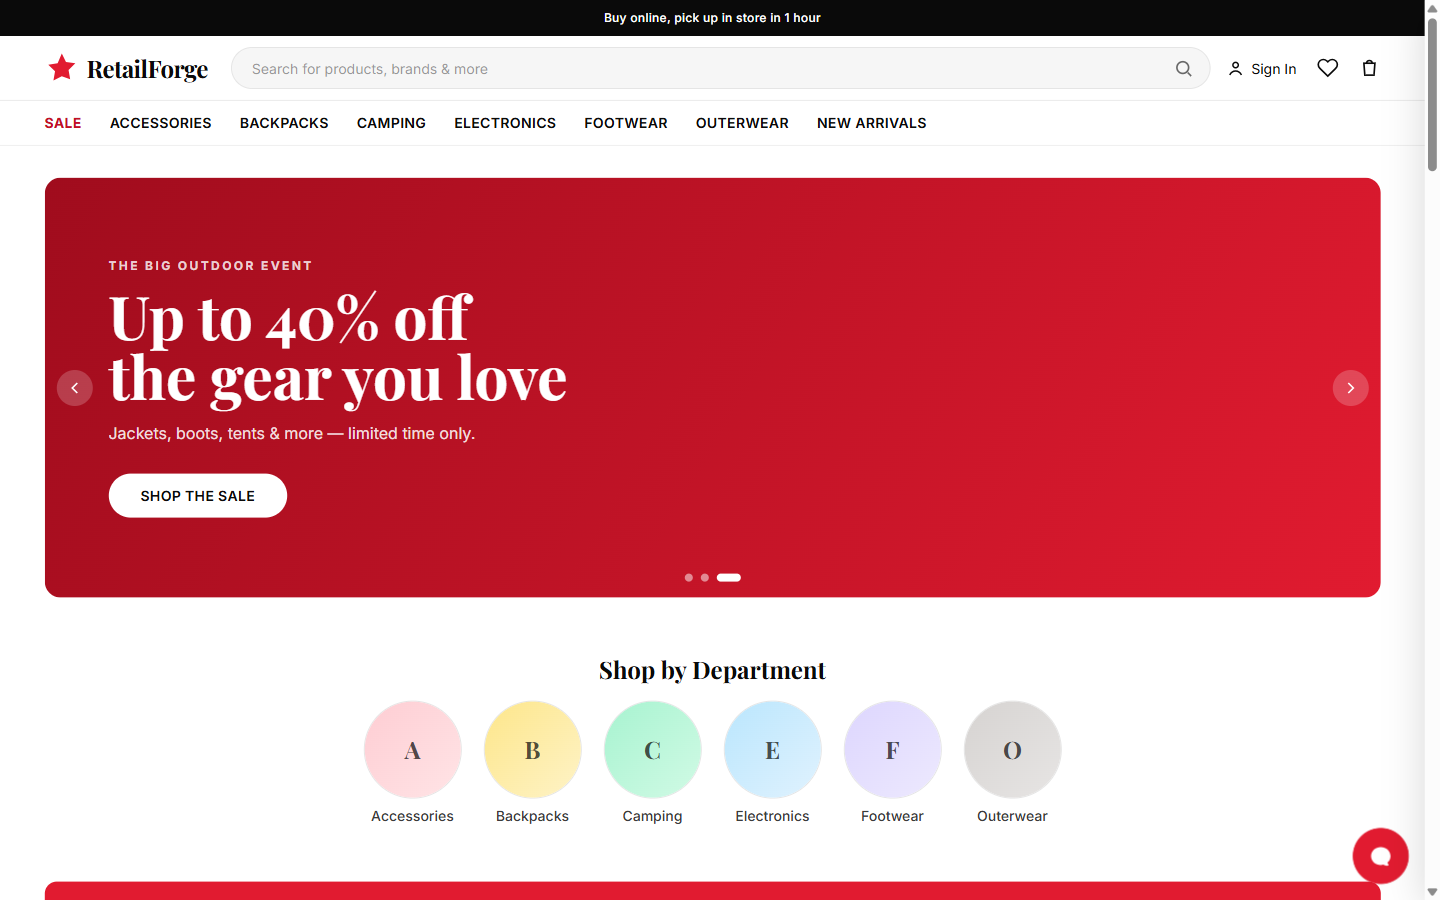
\includegraphics[width=\textwidth]{home-hero.png}};
  \end{tikzpicture}
\end{column}
\begin{column}{0.38\textwidth}
  \small
  A polished \textbf{department-store} experience built in Next.js 15 + Tailwind:
  \begin{itemize}
    \item Hero carousel, department tiles, product rails.
    \item Rich product pages: reviews, stock by aisle, size/color.
    \item Wishlist, bag, and an order history page.
  \end{itemize}
  \vspace{0.3em}
  {\color{ink70}\footnotesize The red star wordmark, serif display type and bold sale
  banners give it an unmistakable retail-floor feel.}
\end{column}
\end{columns}
\end{frame}

% ===================== 5. CONCIERGE IN ACTION ========================
\begin{frame}{The concierge in action --- generative UI}
\begin{columns}[c]
\begin{column}{0.6\textwidth}
  \begin{tikzpicture}
    \node[inner sep=0,draw=line,line width=0.6pt] {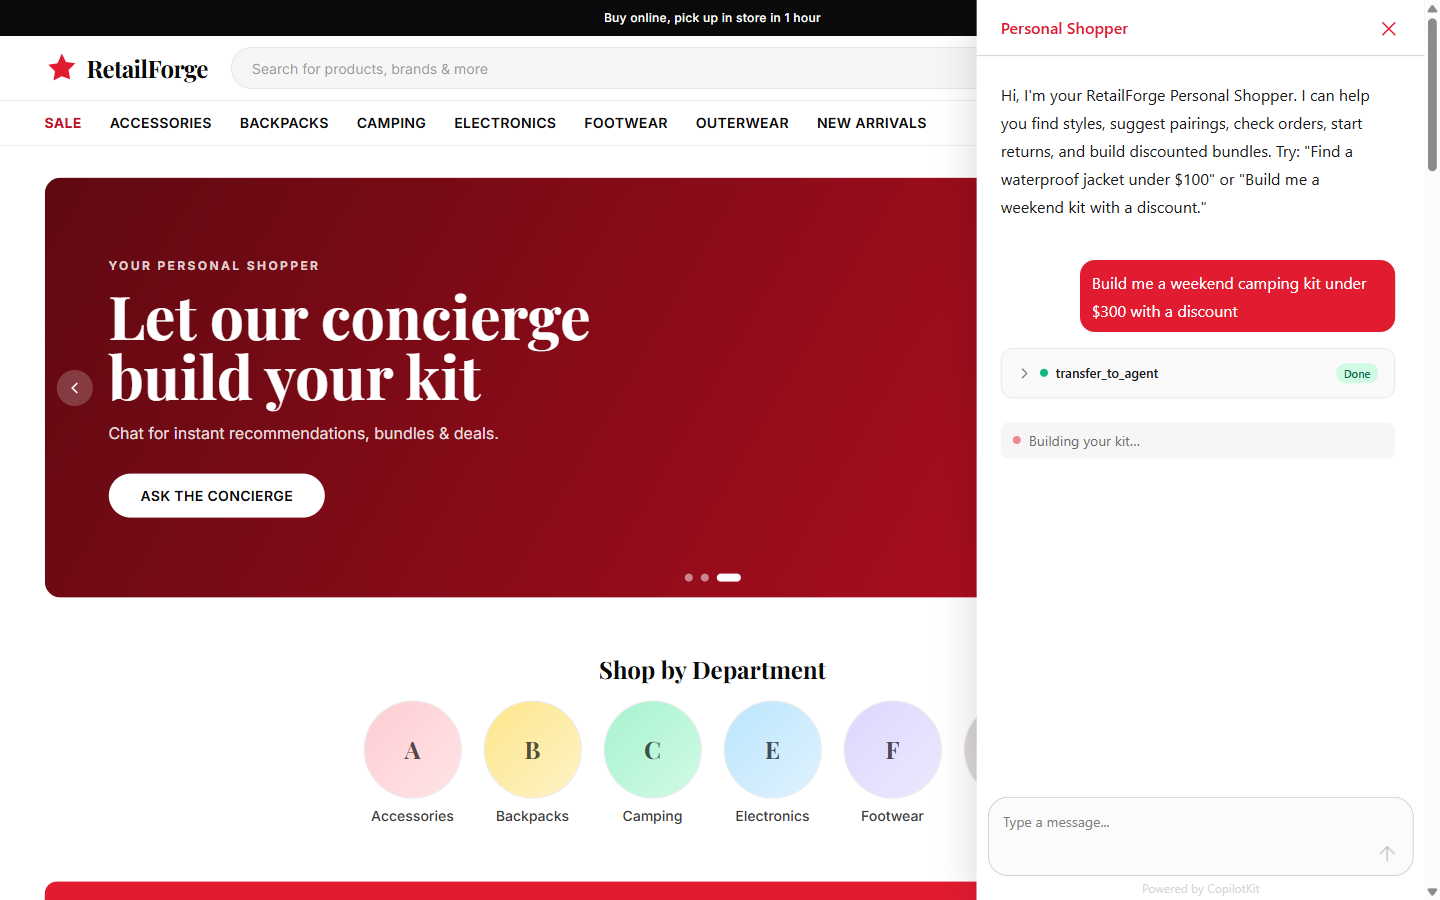
\includegraphics[width=\textwidth]{concierge-chat.png}};
  \end{tikzpicture}
\end{column}
\begin{column}{0.4\textwidth}
  \small
  Powered by \textbf{CopilotKit} over the \textbf{AG-UI} protocol (server-sent events):
  \begin{itemize}
    \item The root agent visibly \texttt{transfer\_to\_agent} to a specialist\dots
    \item \dots which streams \textbf{generative-UI cards}: product grids, kit builder,
          order confirmations, discount results.
    \item Every card has live "Add to Bag" actions wired to the same state as the store.
  \end{itemize}
  \vspace{0.3em}
  {\color{macyred}\footnotesize Captured live --- the agent hand-off is real, not a mock.}
\end{column}
\end{columns}
\end{frame}

% ===================== 6. ARCHITECTURE (TikZ hero) ===================
\begin{frame}{System architecture --- four Cloud Run services}
\centering
\resizebox{!}{6.1cm}{%
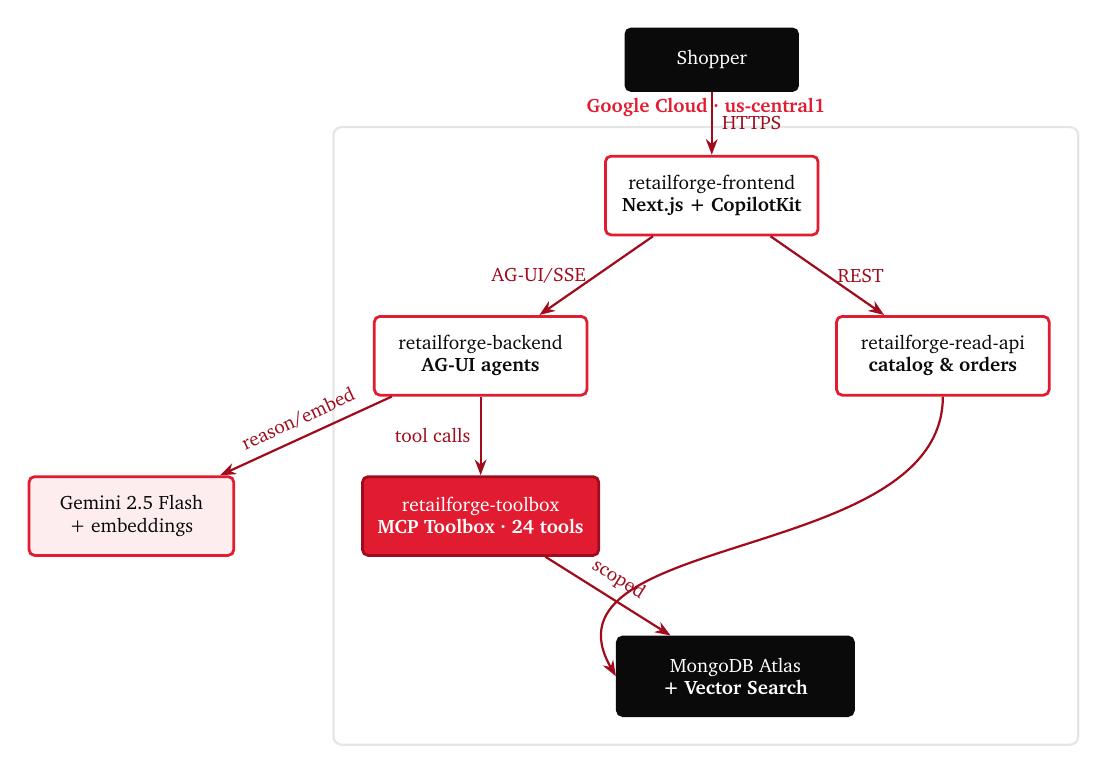
\begin{tikzpicture}[
  font=\scriptsize,
  svc/.style={draw=macyred,line width=1pt,fill=white,rounded corners=2pt,
              align=center,minimum width=2.7cm,minimum height=1.0cm,text=ink},
  tool/.style={draw=macydark,line width=1pt,fill=macyred,rounded corners=2pt,
               align=center,minimum width=3.0cm,minimum height=1.0cm,text=white},
  data/.style={draw=ink,line width=1pt,fill=ink,align=center,
               minimum width=3.0cm,minimum height=1.0cm,text=white,rounded corners=2pt},
  ai/.style={draw=macyred,line width=1pt,fill=macyred!8,rounded corners=2pt,
             align=center,minimum width=2.6cm,minimum height=1.0cm,text=ink},
  user/.style={draw=ink,fill=ink,text=white,rounded corners=2pt,
               minimum width=2.2cm,minimum height=0.8cm},
  flow/.style={-{Stealth[length=2mm]},macydark,line width=0.8pt},
  dash/.style={-{Stealth[length=2mm]},gray,line width=0.6pt,dashed},
]
  \node[user] (u) {Shopper};
  \node[svc,below=0.8cm of u] (fe) {retailforge-frontend\\\textbf{Next.js + CopilotKit}};
  \node[svc,below left=1.0cm and 0.2cm of fe] (be) {retailforge-backend\\\textbf{AG-UI agents}};
  \node[svc,below right=1.0cm and 0.2cm of fe] (read) {retailforge-read-api\\\textbf{catalog \& orders}};
  \node[tool,below=1.0cm of be] (tb) {retailforge-toolbox\\\textbf{MCP Toolbox · 24 tools}};
  \node[ai,left=1.6cm of tb] (gem) {Gemini 2.5 Flash\\+ embeddings};
  \node[data,below right=1.0cm and 0.2cm of tb] (db) {MongoDB Atlas\\\textbf{+ Vector Search}};

  \draw[flow] (u) -- (fe) node[midway,right]{HTTPS};
  \draw[flow] (fe) -- (be) node[midway,left]{AG-UI/SSE};
  \draw[flow] (fe) -- (read) node[midway,right]{REST};
  \draw[flow] (be) -- (gem) node[midway,above,sloped]{reason/embed};
  \draw[flow] (be) -- (tb) node[midway,left]{tool calls};
  \draw[flow] (tb) -- (db) node[midway,above,sloped]{scoped};
  \draw[flow] (read.south) to[out=-90,in=120] (db.west);

  \begin{scope}[on background layer]
    \node[draw=line,line width=0.8pt,rounded corners=3pt,fit=(fe)(be)(read)(tb)(db),
      inner sep=10pt,label={[text=macyred,font=\scriptsize\bfseries]above:Google Cloud · us-central1}] {};
  \end{scope}
\end{tikzpicture}%
}
\par\vspace{0.3em}
{\color{ink70}\scriptsize Each service is independently deployable; secrets are injected from
Secret Manager, images from Artifact Registry.}
\end{frame}

% ===================== 7. MULTI-AGENT ORCHESTRATION ==================
\begin{frame}{Multi-agent orchestration}
\begin{columns}[c]
\begin{column}{0.52\textwidth}
  \centering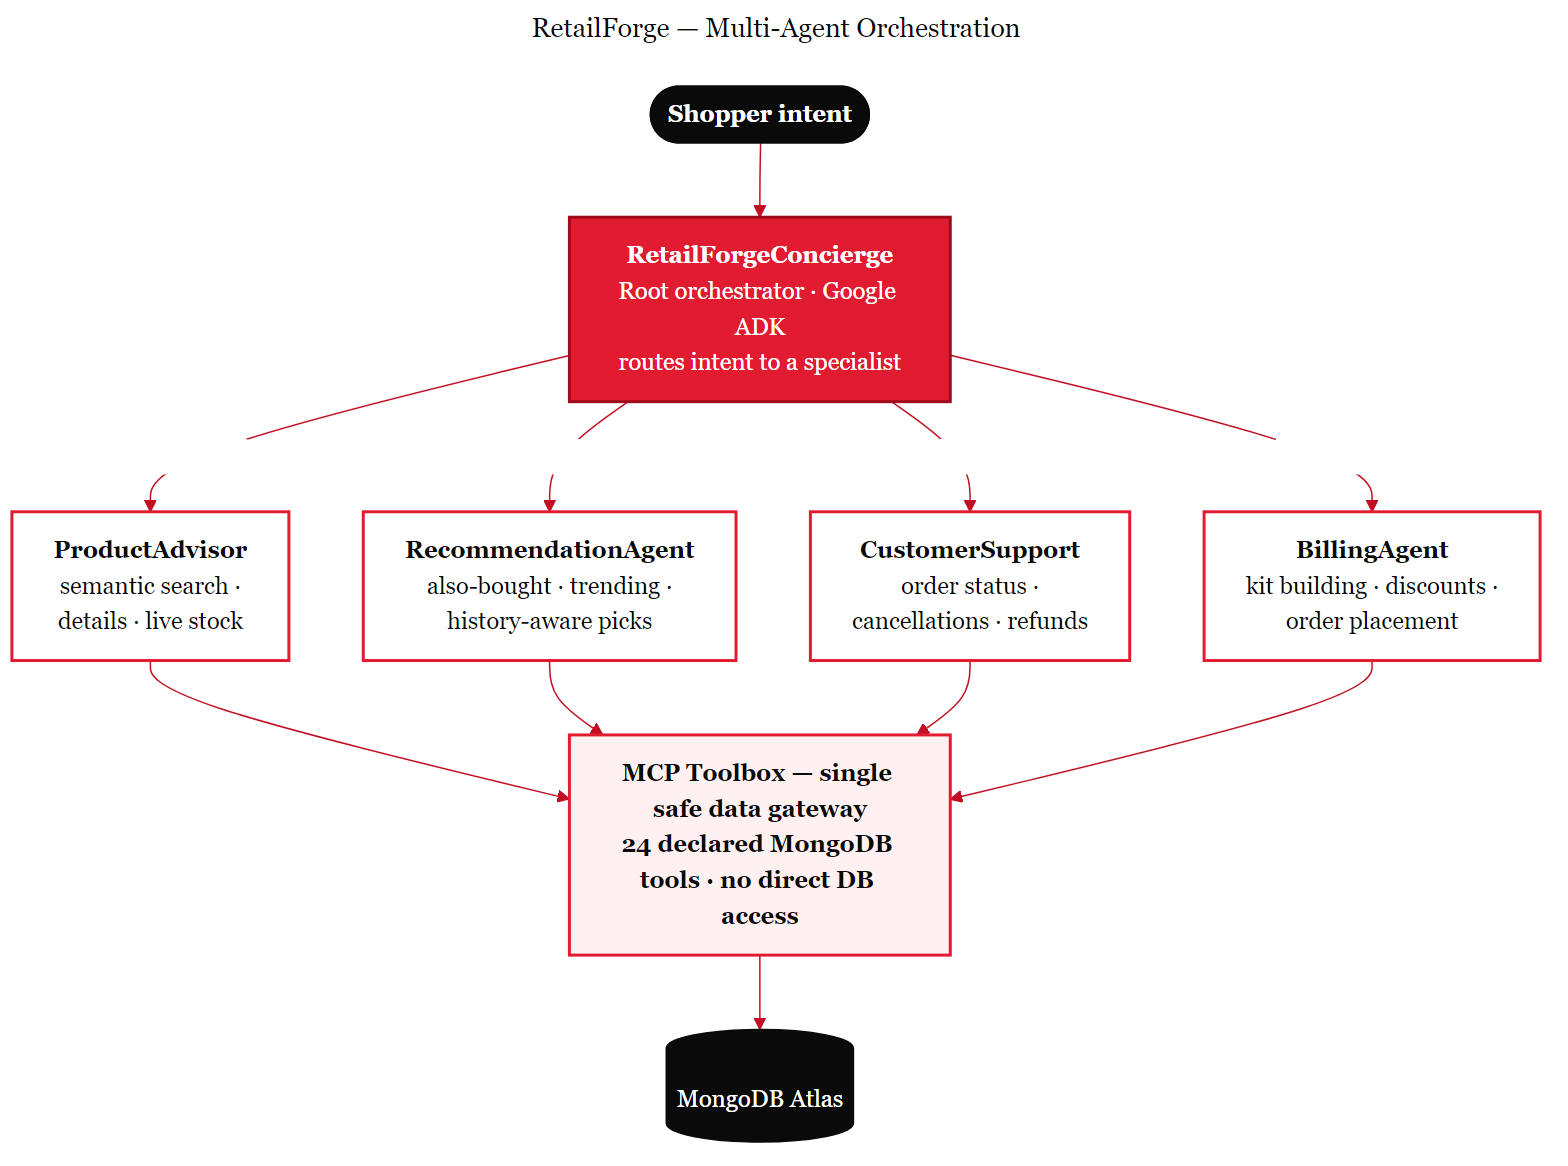
\includegraphics[width=\textwidth]{agents.png}
\end{column}
\begin{column}{0.48\textwidth}
  \small
  A \textbf{root concierge} (Google ADK) classifies intent and hands off to a specialist:
  \begin{itemize}
    \item \textbf{ProductAdvisor} --- search, details, live stock.
    \item \textbf{Recommendation} --- co-purchase, trending, personalization.
    \item \textbf{CustomerSupport} --- status, cancel, refund.
    \item \textbf{Billing} --- kit building, discounts, order placement.
  \end{itemize}
  \vspace{0.3em}
  {\color{ink70}\footnotesize Strategy lives in the LLM; deterministic math
  (pricing, discounts, inventory) stays in native code --- not left to the model.}
\end{column}
\end{columns}
\end{frame}

% ===================== 8. MCP TOOLBOX (key idea) =====================
\begin{frame}{The key idea --- MCP Toolbox as a safety boundary}
\begin{columns}[T]
\begin{column}{0.5\textwidth}
  \textbf{\color{macyred}Agents never open a database connection.}
  \vspace{0.3em}
  \begin{itemize}
    \item Every data operation is a \textbf{declared tool} in \texttt{tools.yaml}.
    \item 24 tools, grouped into 4 toolsets --- one per specialist agent.
    \item An agent can only call what's declared: no ad-hoc, no "DROP".
  \end{itemize}
\end{column}
\begin{column}{0.5\textwidth}
  \textbf{\color{macyred}Why it matters}
  \vspace{0.3em}
  \begin{itemize}
    \item \textbf{Auditable} --- every write is a named, logged tool call.
    \item \textbf{Least privilege} --- read tools and write tools are explicit.
    \item \textbf{Clean contract} --- the model and the system of record are decoupled.
  \end{itemize}
\end{column}
\end{columns}
\vfill
\begin{center}
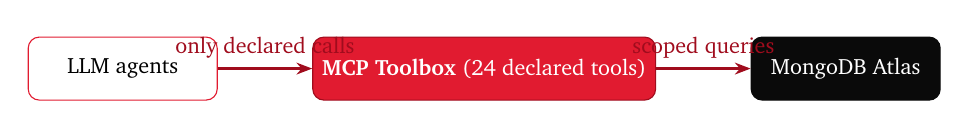
\begin{tikzpicture}[font=\footnotesize,node distance=4mm]
  \node[draw=macyred,fill=white,rounded corners,minimum height=0.8cm,minimum width=2.4cm] (a) {LLM agents};
  \node[draw=macydark,fill=macyred,text=white,rounded corners,minimum height=0.8cm,
        minimum width=3.6cm,right=1.2cm of a] (t) {\textbf{MCP Toolbox} (24 declared tools)};
  \node[draw=ink,fill=ink,text=white,rounded corners,minimum height=0.8cm,
        minimum width=2.4cm,right=1.2cm of t] (d) {MongoDB Atlas};
  \draw[-{Stealth[length=2mm]},macydark,line width=0.9pt] (a) -- (t)
        node[midway,above]{only declared calls};
  \draw[-{Stealth[length=2mm]},macydark,line width=0.9pt] (t) -- (d)
        node[midway,above]{scoped queries};
\end{tikzpicture}
\end{center}
\end{frame}

% ===================== 9. SEMANTIC SEARCH ============================
\begin{frame}{Semantic search \& the action data-flow}
\begin{columns}[c]
\begin{column}{0.58\textwidth}
  \centering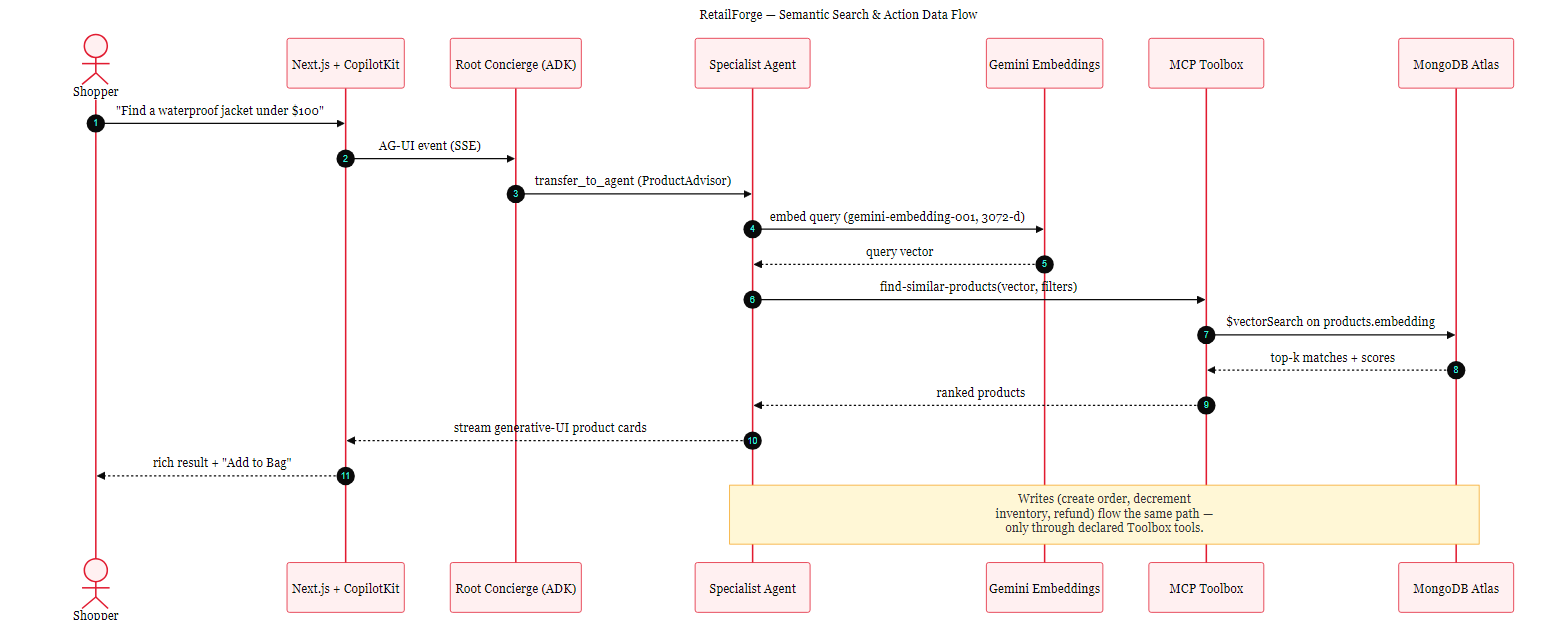
\includegraphics[width=\textwidth]{dataflow.png}
\end{column}
\begin{column}{0.42\textwidth}
  \small
  \begin{itemize}
    \item Products embedded at seed time with \texttt{gemini-embedding-001}
          (\textbf{3072-d}, cosine).
    \item Queries embedded at run time; \textbf{Atlas \$vectorSearch} returns top matches
          with score + metadata filters (category, brand, price).
    \item \textbf{Writes} (create order, decrement inventory, refund) travel the
          \emph{same} gated Toolbox path.
  \end{itemize}
\end{column}
\end{columns}
\end{frame}

% ===================== 10. DATA MODEL ================================
\begin{frame}{Data model --- one Atlas database}
\centering
\renewcommand{\arraystretch}{1.25}
\begin{tabular}{>{\bfseries}l l}
\arrayrulecolor{line}\toprule
\rowcolor{macyred}\textcolor{white}{Collection} & \textcolor{white}{Holds} \\
\midrule
products    & catalog + \textbf{embedding} vector (Vector Search index) \\
\rowcolor{surface}
inventory   & qty on hand, aisle (decremented on order) \\
orders      & line items, subtotal, discount, status, refunds \\
\rowcolor{surface}
reviews     & ratings \& text, aggregated per product \\
promotions  & codes: percentage / fixed, min subtotal, min items \\
\rowcolor{surface}
users       & shopper profiles \\
carts       & abandoned-cart items \\
\bottomrule
\end{tabular}
\par\vspace{0.6em}
{\color{ink70}\footnotesize Vertical-agnostic: swap \texttt{data/sample/*.json} to retarget
the whole store to any retail category.}
\end{frame}

% ===================== 11. DEPLOYMENT ================================
\begin{frame}{Cloud-native deployment}
\begin{columns}[T]
\begin{column}{0.5\textwidth}
\textbf{\color{macyred}Four Cloud Run services}
\begin{itemize}
  \item \textbf{frontend} --- Next.js storefront.
  \item \textbf{backend} --- FastAPI AG-UI agent server.
  \item \textbf{read-api} --- FastAPI catalog/orders.
  \item \textbf{toolbox} --- distroless MCP Toolbox binary.
\end{itemize}
\vspace{0.4em}
\textbf{\color{macyred}Managed building blocks}
\begin{itemize}
  \item Secret Manager --- Mongo URI \& Gemini key.
  \item Artifact Registry --- SHA-tagged images.
\end{itemize}
\end{column}
\begin{column}{0.5\textwidth}
\textbf{\color{macyred}Infrastructure as code}
\begin{itemize}
  \item \textbf{Terraform} provisions all services, secrets \& IAM.
  \item Remote state in GCS --- repeatable applies.
  \item One \texttt{terraform apply} stands up the whole stack.
\end{itemize}
\vspace{0.4em}
\begin{block}{Live URLs}
\scriptsize
frontend / backend / read-api / toolbox\\
\texttt{retailforge-*-awghszkm2a-uc.a.run.app}
\end{block}
\end{column}
\end{columns}
\end{frame}

% ===================== 12. CI/CD ====================================
\begin{frame}{CI/CD --- push to production, keyless}
\centering
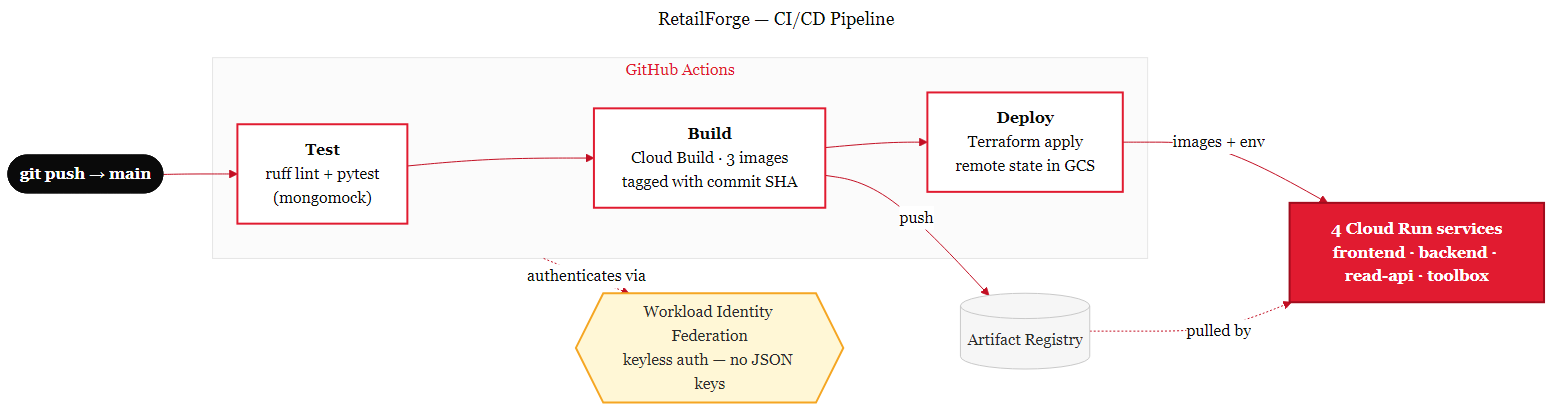
\includegraphics[width=0.96\textwidth]{cicd.png}
\par\vspace{0.4em}
\small
\textbf{GitHub Actions}: test (ruff + pytest on mongomock) $\rightarrow$ Cloud Build (3 images,
commit-SHA tags) $\rightarrow$ Terraform apply. Auth via \textbf{Workload Identity Federation}
--- \emph{no service-account JSON keys in the repo}.
\end{frame}

% ===================== 13. TECH STACK ===============================
\begin{frame}{Tech stack}
\centering
\renewcommand{\arraystretch}{1.22}
\begin{tabular}{>{\bfseries}l l}
\arrayrulecolor{line}\toprule
\rowcolor{macyred}\textcolor{white}{Layer} & \textcolor{white}{Technology} \\
\midrule
Frontend       & Next.js 15, React 19, TypeScript, Tailwind, CopilotKit, AG-UI \\
\rowcolor{surface}
Agents         & Google ADK, ag-ui-adk, Gemini 2.5 Flash \\
Backend        & FastAPI, Uvicorn, Pydantic \\
\rowcolor{surface}
Data           & MongoDB Atlas + Vector Search, gemini-embedding-001 (3072-d) \\
Tooling        & MCP Toolbox (genai-toolbox), toolbox-core \\
\rowcolor{surface}
Infra          & Cloud Run, Secret Manager, Artifact Registry, Cloud Build \\
IaC \& CI/CD    & Terraform, GitHub Actions, Workload Identity Federation \\
\rowcolor{surface}
Quality        & pytest, mongomock, ruff \\
\bottomrule
\end{tabular}
\end{frame}

% ===================== 14. MORE SCREENS =============================
\begin{frame}{More of the experience}
\centering
\begin{tikzpicture}
  \node[inner sep=0,draw=line] (a)
    {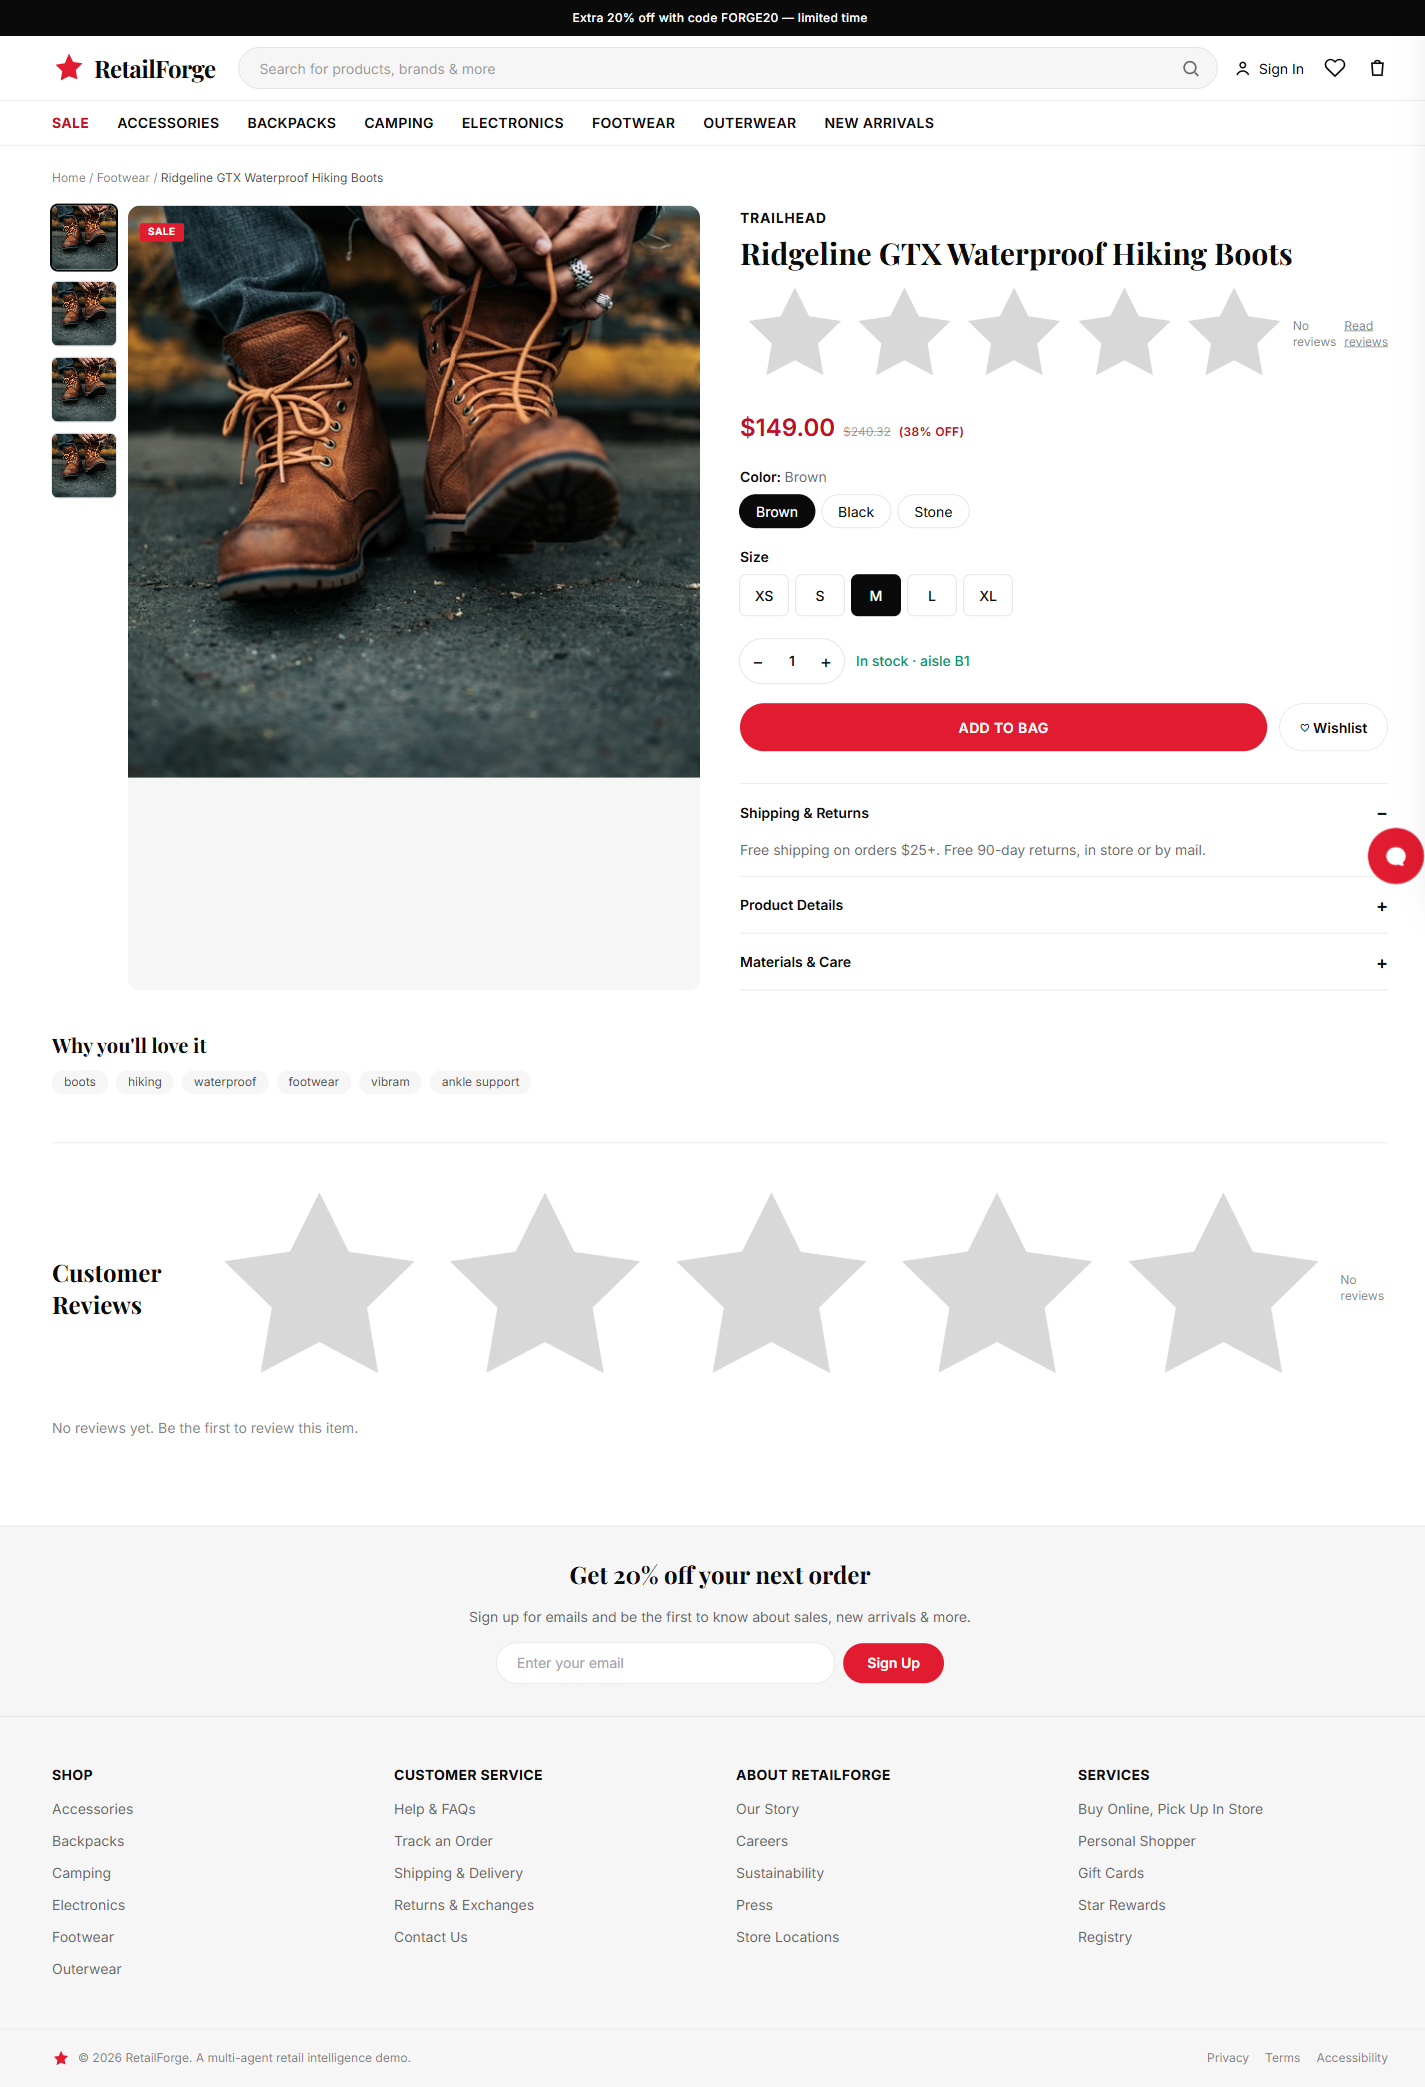
\includegraphics[height=5.4cm]{product-detail.png}};
  \node[inner sep=0,draw=line,right=0.5cm of a] (b)
    {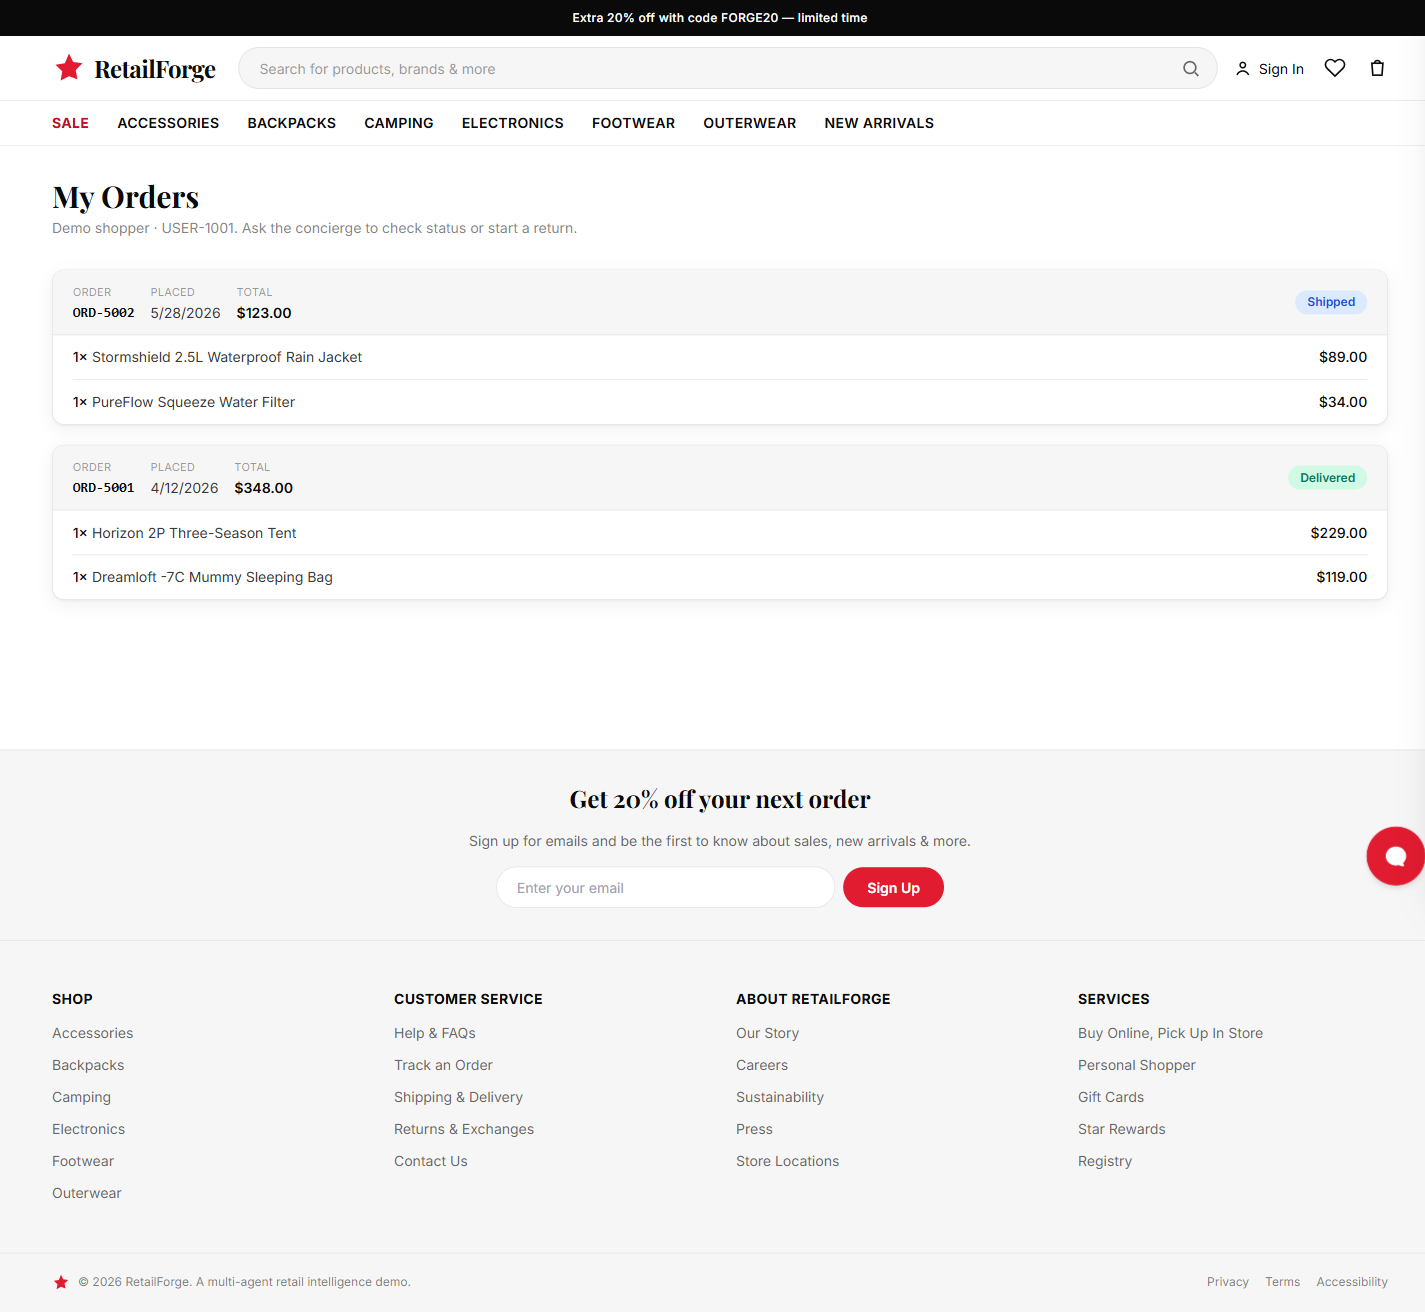
\includegraphics[height=5.4cm]{orders.png}};
  \node[inner sep=0,draw=line,right=0.5cm of b] (c)
    {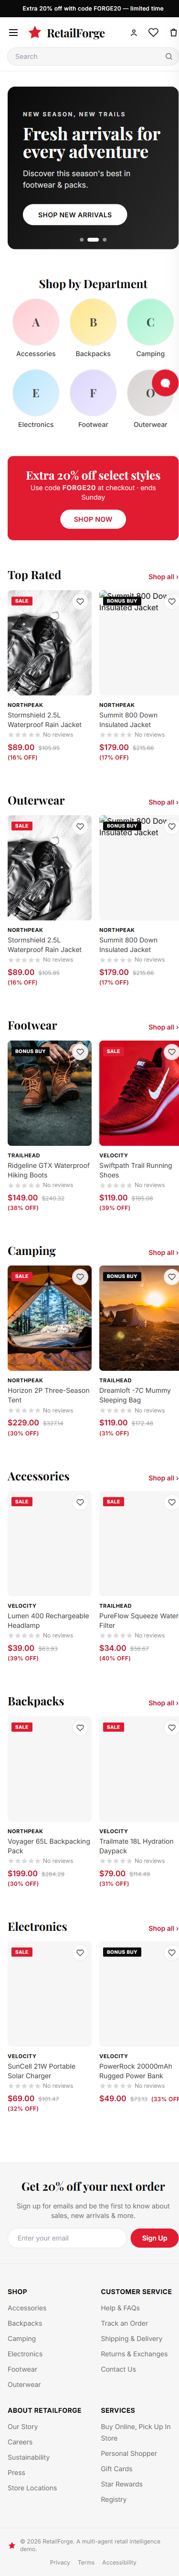
\includegraphics[height=5.4cm]{home-mobile.png}};
\end{tikzpicture}
\par\vspace{0.3em}
{\color{ink70}\footnotesize Product detail with reviews \& live stock \quad$\cdot$\quad
order history with status badges \quad$\cdot$\quad fully responsive mobile.}
\end{frame}

% ===================== 15. CHALLENGES ===============================
\begin{frame}{Challenges \& what we learned}
\begin{columns}[T]
\begin{column}{0.5\textwidth}
\textbf{\color{macyred}Challenges}
\begin{itemize}
  \item Keeping agents from touching data directly --- solved with the Toolbox boundary.
  \item Tuning vector search relevance (task-type, filters, top-k).
  \item Running a \textbf{distroless} Toolbox on Cloud Run (no shell, direct binary, port 8080).
  \item Boot ordering: make Toolbox public \emph{before} the backend loads its tools.
\end{itemize}
\end{column}
\begin{column}{0.5\textwidth}
\textbf{\color{macyred}Learnings}
\begin{itemize}
  \item Let the \textbf{LLM strategize}; keep money math in deterministic code.
  \item A declared-tool layer makes agent actions \emph{auditable by construction}.
  \item Generative UI beats plain chat --- actions live where the answer is.
  \item Keyless WIF + Terraform = clean, repeatable, secret-free deploys.
\end{itemize}
\end{column}
\end{columns}
\end{frame}

% ===================== 16. WHAT'S NEXT / CLOSE ======================
{%
\setbeamertemplate{footline}{}
\begin{frame}[plain]
\begin{tikzpicture}[remember picture,overlay]
  \fill[macyred] (current page.south west) rectangle (current page.north east);
  \node[anchor=north west] at ([xshift=1.1cm,yshift=-1.0cm]current page.north west){\titlestar};
  \node[anchor=west,white,font=\LARGE\bfseries] at
      ([xshift=2.6cm,yshift=-1.6cm]current page.north west){What's next};
  \node[anchor=north west,white,font=\normalsize] at
      ([xshift=1.15cm,yshift=-3.2cm]current page.north west)
      {\parbox{12cm}{\raggedright
        \begin{itemize}
          \item Tighten IAM (auth'd service-to-service) + VPC egress for static Atlas IPs.
          \item Personalization from real session \& purchase history.
          \item Payment + fulfillment integration; A/B test agent strategies.
          \item Observability: trace every agent hand-off and tool call.
        \end{itemize}}};
  \node[anchor=south west,white,font=\small] at
      ([xshift=1.15cm,yshift=1.5cm]current page.south west)
      {\parbox{12cm}{\raggedright \textbf{Try it live:}
       retailforge-frontend-awghszkm2a-uc.a.run.app}};
  \node[anchor=south east,white,font=\Large\bfseries] at
      ([xshift=-1.1cm,yshift=1.2cm]current page.south east){Thank you \ \macystar[white]{4pt}};
\end{tikzpicture}
\end{frame}
}

\end{document}
